% !TEX program = xelatex
% !TEX encoding = UTF-8
% ================================================================
%  Harness：大模型智能体执行框架的设计空间与工程评测
%  —— LaTeX 版初稿（2026-10-05）· 排版格式化版
%  说明：本次仅做版式与源码格式整理，正文内容未改动。
%
%  编译要求：必须使用 XeLaTeX（中文排版 + 字体）
%   · Overleaf：上传本文件 → Menu → Compiler → XeLaTeX → Recompile
%   · 本地：latexmk -xelatex harness-paper.tex（需 TeX Live / MiKTeX）
%
%  依赖宏包（均为标准 TeX 发行版自带）：
%   ctexart, geometry, amsmath, amssymb, booktabs, tabularx, array,
%   enumitem, graphicx, xcolor, tikz, caption, hyperref
% ================================================================
\documentclass[11pt,a4paper]{ctexart}

% ---------- 版式与页面 ----------
\usepackage{geometry}
\geometry{left=2.5cm,right=2.5cm,top=2.8cm,bottom=2.8cm}

% ---------- 数学 ----------
\usepackage{amsmath,amssymb}

% ---------- 表格与列表 ----------
\usepackage{booktabs}
\usepackage{tabularx}
\usepackage{array}
\usepackage{enumitem}
\setlist{itemsep=2pt,topsep=3pt,parsep=0pt}

% ---------- 图形与颜色 ----------
\usepackage{graphicx}
\usepackage{xcolor}
\usepackage{tikz}
\usetikzlibrary{arrows.meta,positioning,fit,backgrounds}
\usepackage{caption}
\captionsetup{font=small,labelfont=bf,skip=6pt}

% ---------- 超链接（建议最后加载） ----------
\usepackage{hyperref}
\hypersetup{colorlinks=true,linkcolor=blue!55!black,citecolor=blue!55!black,urlcolor=blue!55!black}

% ---------- 全局排版微调 ----------
\renewcommand{\arraystretch}{1.15}
\setlength{\emergencystretch}{2em}

\title{\bfseries Harness：大模型智能体执行框架的设计空间与工程评测\\[5pt]
       \large ——以 DeepSeek Harness 为案例的多框架对比研究}
\author{（作者署名待补）\\[3pt]
        \small 稿件类型：分析论文（Position \& Analysis Paper）；初稿}
\date{2026 年 10 月 5 日}

\begin{document}

\maketitle

\begin{center}
\small\itshape
Harness: Design Space and Engineering Evaluation of LLM Agent Execution Frameworks\\
--- A Comparative Study Centered on DeepSeek Harness
\end{center}

\begin{quote}
\small\textbf{写作声明}：第 5 章的对比评分为基于公开资料的定性分析，非受控实验测量值；参考文献为写作时整理，正式使用前应逐条联网核验（本工作区 \texttt{Sources.md} 记录的方法论可作核验起点）。
\end{quote}

\begin{abstract}
大语言模型（LLM）的基础能力近年来持续跃升，但从“会对话”到“能自主完成复杂任务”之间仍横亘着一道工程鸿沟。填补这道鸿沟的关键软件层被本文统称为 \textbf{Harness}（智能体执行框架）——它包裹在模型之外，赋予智能体以工具调用、循环控制、上下文管理、权限约束与扩展能力。本文围绕三个问题展开：（RQ1）Harness 的功能结构应如何刻画？（RQ2）以“万物皆插件”（Everything is a Plugin）为理念的 DeepSeek Harness 代表了怎样一种架构取向，其收益与代价为何？（RQ3）面对接口与形态各异的多种 Harness，如何建立可比的评测框架？针对 RQ1，本文提出“工具接口—循环编排—上下文管理—权限安全—扩展生态”五维设计空间；针对 RQ2，本文以 DeepSeek 开源项目 DeepSeek Harness 为中心案例，结合 Claude Code、OpenAI Codex、Notrat、OpenHands 等代表性框架展开结构化对比；针对 RQ3，本文提出“模型×框架”解耦归因原则与 L1--L4 分层评测框架，并给出可执行的实证研究提案。分析表明：插件化解耦程度、上下文分层管理与安全沙箱强度是决定 Harness 工程价值的三个主导因素；智能体系统的成功率应归因于模型与框架的乘积效应，而非任何单一来源。
\end{abstract}

\medskip
\noindent\textbf{关键词}：大语言模型；智能体；执行框架；Harness；插件化架构；工具调用；模型上下文协议

\section{引言}

\subsection{从“裸模型”到“能干的智能体”}

以 GPT、Claude、DeepSeek 等为代表的大语言模型展现出强大的语言理解、推理与代码生成能力。然而，将模型直接置入真实工作场景后，差距很快显现：它可以写出漂亮的函数，却无法自行打开项目、定位文件、修改代码并跑通测试；它可以规划出合理的步骤，却难以在数十步之后仍然记得自己的进度与约束。

学术界很早就意识到“行动能力”需要外部机制补足。ReAct（Yao et al., 2023）提出“推理—行动”交替范式，让模型在思考与调用工具之间循环；Toolformer（Schick et al., 2023）展示了模型自学调用外部 API 的可行性；Voyager（Wang et al., 2023）在开放环境中验证了“模型 + 执行环境 + 记忆”组合的威力。这些工作的共同指向是：\textbf{模型的能力边界不仅是参数量的函数，也是其所处执行框架的函数。}

本文将这一执行框架统称为 \textbf{Harness}。

\subsection{问题：差异不只在模型}

工业实践提供了最直观的证据：同一模型家族在不同产品形态（终端 CLI、IDE 插件、桌面工作台、云端服务）中的表现差异显著；以近似模型能力构建的不同编码智能体，其可靠性、可控性与扩展性也大相径庭。这提示我们：\textbf{当模型能力趋同时，产品差异的主战场已从模型层转移到 Harness 层。}

由此，本文提出三个研究问题：

\begin{itemize}
  \item \textbf{RQ1（结构）}：Harness 由哪些功能层构成？各层的设计轴与权衡是什么？
  \item \textbf{RQ2（架构）}：以“万物皆插件”为理念的 DeepSeek Harness 代表了怎样的架构取向？其收益、代价与适用边界为何？
  \item \textbf{RQ3（评测）}：面对接口、形态、协议各异的多种 Harness，如何建立可比的评测框架？
\end{itemize}

\subsection{本文贡献}

\begin{enumerate}
  \item \textbf{框架贡献}：提出 Harness 五维设计空间（工具接口 / 循环编排 / 上下文管理 / 权限安全 / 扩展生态），给出各维度的设计轴与典型权衡；
  \item \textbf{案例贡献}：以 DeepSeek Harness 为中心案例，对照 Claude Code、OpenAI Codex、Notrat、OpenHands，形成覆盖 7 项特征的结构化对比；
  \item \textbf{方法贡献}：提出“模型×框架”解耦归因原则与 L1--L4 分层评测框架（能力 / 韧性 / 信任 / 生态），并给出可执行的实证研究提案；
  \item \textbf{议题贡献}：讨论 Harness 领域的三类挑战——可复现性、安全性与基准缺失，并给出未来方向。
\end{enumerate}

\subsection{论文结构}

第 2 章回顾背景与相关工作；第 3 章提出五维设计空间；第 4 章为案例研究；第 5 章给出对比分析与评测框架；第 6 章讨论挑战与未来方向；第 7 章总结全文。

\section{背景与相关工作}

\subsection{“模型 + Harness”命题}

本文将智能体系统的任务成功率形式化地表示为模型与框架的联合函数：

\begin{equation}
P(\text{成功}\mid T) = F\bigl(M(T,H),\, H\bigr)
\label{eq:pair}
\end{equation}

其中 $M$ 表示模型在框架 $H$ 所提供的上下文与工具条件下产生的决策流。式~\eqref{eq:pair} 的工程含义是：\textbf{报告智能体成绩时应同时披露模型版本与框架版本}，否则结果无法归因、无法复现——这一点在当前多数基准报告中普遍缺失。

\subsection{编排范式：从单循环到多智能体}

早期编排以单智能体 ReAct 循环为主。随后出现以“多角色协作”为核心的框架：AutoGen（Wu et al., 2023）提出可对话的智能体集合；MetaGPT（Hong et al., 2024）将软件流程编码为角色分工；ChatDev（Qian et al., 2023）以“虚拟软件公司”隐喻组织协作；Generative Agents（Park et al., 2023）则探索了长期记忆与社会行为的涌现。这些工作探明了分工的价值，也暴露了通信开销与错误传播的问题。近期工业界 Harness 的共识倾向于：\textbf{单代理主循环 + 子代理按需分派}的混合结构在工程上更为稳健。

\subsection{工业 Harness 谱系}

\begin{itemize}
  \item \textbf{Claude Code（Anthropic）}：终端原生编码智能体，以项目约定文件（CLAUDE.md）、权限审批与钩子（hooks）机制为特色；
  \item \textbf{OpenAI Codex}：开源编码智能体（Rust 实现），覆盖 CLI / IDE / 桌面 / 云端四种形态，以本地沙箱 + 审批、AGENTS.md 约定与云端 PR 工作流为特色；
  \item \textbf{DeepSeek Harness（dsh）}：DeepSeek 开源的执行框架，基于 Cordis 插件运行时构建；核心理念为 “Everything is a Plugin”（万物皆插件），主张内核极薄、一切能力以插件形式装配；目前处于开发者预览（developer preview）阶段；
  \item \textbf{OpenHands（原 OpenDevin）}：社区开源智能体平台，强调沙箱化的可复现执行；
  \item \textbf{Notrat}：本地优先的桌面工作台形态，将写作、Agent 运行时、终端与自动化（定时任务 / IM 网关 / 多端同步）整合于一体，支持 MCP 与外部 CLI 接入。
\end{itemize}

\subsection{标准化层：MCP 与约定文件}

Model Context Protocol（MCP，Anthropic 于 2024 年开源）试图统一“模型→工具”的连接方式，降低每个 Harness 重复适配工具的成本；AGENTS.md、CLAUDE.md 等约定文件把“项目级知识”从散落的提示词中抽出，变为可版本化的仓库资产。标准化层的出现，标志着 Harness 进入“接口收敛”阶段。

\subsection{评测现状与缺口}

SWE-bench（Jimenez et al., 2024）等基准以“任务完成”为度量，极大推动了编码智能体的可比性。但现有基准普遍将模型与框架\textbf{绑定为单一系统}进行报告。作为研究对象的 Harness 本身——其架构决策如何影响可靠性、安全与成本——仍缺乏系统性文献。本文的定位正是补上这一层。

\section{Harness 设计空间：五维框架}

本章对应 \textbf{RQ1}，提出五维框架（图~\ref{fig:five-dim}）。

\begin{figure}[htbp]
  \centering
  % 图形已抽成独立源文件 figs/fig-five-dim.tex（standalone 类），下面引入它的编译产物。
  % 改图请改 fig-five-dim.tex —— 不要再把 tikzpicture 内联回来。
  % 重新导出：bash figs/build.sh   （或在插件设置里把编译引擎换成 latexmk，见 samples/latexmkrc）
  % ⚠ 扩展名必须写成 .pdf：figs/ 下同时有同名 .tex（图源），
  %   不带扩展名时预览的资产通道会先命中那个 .tex，把图当文本读，图就不显示了。
  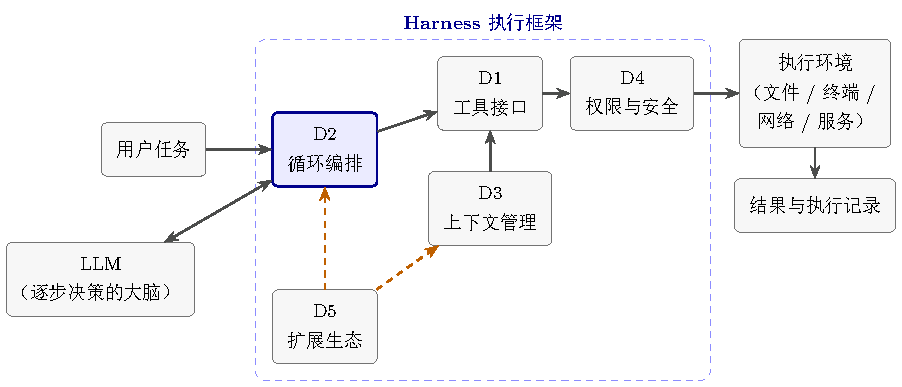
\includegraphics[width=\textwidth]{figs/fig-five-dim.pdf}
  \caption{Harness 五维结构示意（D1--D5 对应下文各小节；虚线框为执行框架范围，橙色虚线示意扩展生态的插拔式接入）。}
  \label{fig:five-dim}
\end{figure}

\subsection{维度一：工具接口层（Tool Interface）}

工具是智能体的“手脚”。设计轴包括：

\begin{itemize}
  \item \textbf{内置 vs 外挂}：内置工具（文件、终端、搜索、浏览器）保证开箱可用；MCP 等协议支持外挂第三方工具；
  \item \textbf{工具粒度}：粗粒度（“完成一次重构”）减少决策步数、提升效率，但降低可控性；细粒度反之；
  \item \textbf{可组合性}：工具间能否流式衔接（如“搜索→抓取→整理→写文件”链路）。
\end{itemize}

典型权衡：\textbf{能力 × 可控性}——工具面越宽越强，误用与安全面也越大。

\subsection{维度二：循环编排层（Loop \& Orchestration）}

\begin{itemize}
  \item \textbf{单循环 vs 多阶段}：ReAct 式单循环结构简单，但长任务中易“迷航”；“计划—执行—验证”多阶段结构提升可靠性，代价是额外开销与刚性；
  \item \textbf{子代理分派}：主代理按需分派独立子任务（调研、检索、审查），既并行加速，又隔离上下文污染；
  \item \textbf{人在环（HITL）}：审批门插入的位置与频度，决定“自动化程度 ↔ 风险”的配比。
\end{itemize}

\subsection{维度三：上下文管理层（Context Management）}

长任务是 Harness 的试金石，而上下文窗口是硬约束。主要机制：

\begin{itemize}
  \item \textbf{压缩}：阈值触发（如上下文用量达 80\% 时压缩）、分层摘要（旧事粗记、近事精记）；
  \item \textbf{检索}：向量 + 关键词混合检索本地知识库，把“记得住”变成“找得到”；
  \item \textbf{外部记忆}：将中间状态写入文件、任务清单等外部载体，避免状态随压缩丢失。
\end{itemize}

设计轴：\textbf{信息保真度 × 成本 × 延迟}。

\subsection{维度四：权限与安全层（Permission \& Safety）}

\begin{itemize}
  \item \textbf{审批模式}：全自动 / 危险操作询问 / 逐条批准；
  \item \textbf{沙箱强度}：目录级（限定工作区）→ 进程级 → 容器级 → 虚拟机级；
  \item \textbf{网络与数据边界}：能否外发请求、哪些数据不得出域；
  \item \textbf{供应链治理}：插件/技能市场的签名、审计与最小权限原则。
\end{itemize}

这是 Harness 区别于“聊天机器人”的核心工程承诺：\textbf{把强大的执行力约束在可预期的边界之内}。

\subsection{维度五：扩展与生态层（Extension \& Ecosystem）}

\begin{itemize}
  \item \textbf{插件化程度}：内核全解耦（一切皆插件）↔ 内核固化（仅外围可扩展）；
  \item \textbf{分发渠道}：包管理器 / 应用内市场 / 仓库直装；
  \item \textbf{多端形态}：CLI / IDE / 桌面 / IM / 云端的一致性体验。
\end{itemize}

核心权衡：\textbf{扩展自由度 ↔ 稳定性与安全}——自由度越高，生态越易繁荣，但质量与安全治理越难。

\subsection{维度间耦合}

五维并非正交：插件化（D5）扩张工具面（D1），进而放大权限风险（D4）；压缩策略（D3）的有效性依赖编排结构（D2）能否将状态外置；沙箱强度（D4）反过来约束可用工具集（D1）。后文的案例分析与评测均沿此五维展开。

\section{案例研究：DeepSeek Harness}

本章对应 \textbf{RQ2}。先给项目概况，再剖析其技术底座（Cordis 与“时空可组合性”范式），随后以五维框架作映射分析。

\subsection{项目概况}

DeepSeek Harness（简称 \textbf{dsh}）是 DeepSeek AI 开源维护的智能体框架，以 MIT 许可发布，官方自述为“构建于\textbf{一切皆插件}（everything-is-a-plugin）架构之上，由 Cordis 驱动”。

主要公开事实（据其 GitHub 仓库，截至 2026-10）：

\begin{itemize}
  \item \textbf{热度}：GitHub 星标约 \textbf{24.4 万}、Fork 约 2.92 万、提交数超过 \textbf{2 万}——在开源 Agent 框架中处于第一梯队；
  \item \textbf{运行}：\texttt{npx @deepseek-ai/dsh web} 一条命令即可在本地 \texttt{127.0.0.1:3080} 启动 Web UI；同时提供桌面端构建目标与 Python SDK（含面向基准评测的 jsonrpc-agent 最小变体）；
  \item \textbf{成熟度}：处于\textbf{开发者预览}（developer preview）阶段，官方明示“将出现破坏兼容性的变更”；运行前需阅读独立的安全说明；
  \item \textbf{社区}：通过 GitHub Discussions、Discord 与国内社群协作；插件以 \texttt{dsh-plugin} 话题约定发现；
  \item \textbf{文档}：独立文档站（架构文档 / 开发指南 / Cordis 教程齐全），并为 AI 协作者准备了 \texttt{AGENTS.md}。
\end{itemize}

\subsection{技术底座：Cordis 与“时空可组合性”}

dsh 的独特之处不在功能清单，而在\textbf{它把 harness 自身当作一个可组合系统来设计}。

其底座 \textbf{Cordis}（拉丁语“心”）是一个 TypeScript 元框架（meta-framework，即“用于构建框架的框架”），核心职责极窄：插件的\textbf{加载、卸载与依赖关系管理}。其设计论文《A Programming Paradigm for Spatiotemporal Composability》（北京大学与 DeepSeek 合作，2026 年 8 月预印本）提出两个正交维度：

\begin{itemize}
  \item \textbf{时间可组合性}（temporal composability）：组件被移除时，能够\textbf{完全撤销}其副作用——即“可逆的插件系统”；
  \item \textbf{空间可组合性}（spatial composability）：组件在作用域与边界上的隔离与组合。
\end{itemize}

论文将上述思想实现为 Cordis：一个只做“可组合性”的极小内核，并把工具调用、LLM 适配、任务流转等智能体能力全部下放给插件。这一思路的工程含义可概括为：\textbf{如果每个插件都能被安全地装上、卸下与替换，则系统永远保持可演进}——这恰是长期运行的智能体系统最稀缺的性质。

\subsection{五维映射与代价分析}

\begin{table}[htbp]
  \centering
  \small
  \caption{DeepSeek Harness 的五维映射与代价分析}
  \label{tab:dsh-map}
  \begin{tabularx}{\textwidth}{l p{4.8cm} X}
    \toprule
    维度 & DeepSeek Harness 的取向 & 对应的收益与代价 \\
    \midrule
    D1 工具接口 & 工具即插件，\texttt{dsh-plugin} 生态约定 & 扩展性极强；需治理插件规范、命名空间与冲突 \\
    D2 循环编排 & 智能体能力（工具调用、LLM 适配、任务流转）全部由插件承载 & 弹性大；默认体验取决于所选插件组合 \\
    D3 上下文管理 & 会话制运行（基准指引要求独立工作区与会话 ID） & 隔离性好、利于评测复现；跨会话记忆需生态补齐 \\
    D4 权限安全 & 携带独立安全声明（\texttt{SAFETY.md}），运行前强制阅读 & 安全是显式工程项；插件供应链治理仍待成熟 \\
    D5 扩展生态 & 解耦程度最高档；元框架级别可组合 & 生态爆发潜力大；预览期兼容性风险高 \\
    \bottomrule
  \end{tabularx}
\end{table}

一句话概括：\textbf{dsh 押注“架构中立性”}——不与特定模型、工具或界面绑定，把差异留给插件生态竞争；并以一篇理论论文为这种取向提供了形式化基础。这与“垂直整合”路线（模型 + 框架 + 产品一体优化）构成一组鲜明的战略对照。

\subsection{同类框架的路线对照}

\begin{itemize}
  \item \textbf{Claude Code}：垂直整合 + 约定文件 + 审批门，追求“开箱即用的可靠性”；
  \item \textbf{OpenAI Codex}：垂直整合 + 强沙箱 + 云端工作流，追求“本地到云端的连续工程体验”；
  \item \textbf{Notrat}：工作台一体化，将知识管理、Agent 与自动化置于同一桌面环境，追求“个人全能生产力”；
  \item \textbf{OpenHands}：平台化 + 沙箱化，面向研究与团队的可复现实验。
\end{itemize}

五者的差异本质上是五维框架上的不同取值组合——这正是第 5 章评测框架要刻画的。

\section{对比分析与评测框架}

本章对应 \textbf{RQ3}。

\subsection{研究对象与选取标准}

选取 5 个代表性框架：DeepSeek Harness、Claude Code、OpenAI Codex、Notrat、OpenHands。选取标准：（a）公开可得且活跃维护；（b）形态覆盖框架库 / CLI / 桌面 / 平台；（c）在“插件化程度”维度形成清晰梯度。

\subsection{结构化对比矩阵}

\begin{quote}
\small\textbf{评分口径}：下表为撰写本文整理的定性分析（★ 为 5 星制），依据为公开文档与仓库信息，\textbf{非受控实验测量}；仅供结构性讨论，不作为选型依据。数据基准：2026-10。
\end{quote}

\begin{table}[htbp]
  \centering
  \small
  \setlength{\tabcolsep}{4pt}
  \caption{五个代表性 Harness 的结构化对比（★ 为五星制定性评分，非实验测量；数据基准：2026-10）}
  \label{tab:compare}
  \begin{tabularx}{\textwidth}{p{2.1cm} *{5}{>{\centering\arraybackslash}X}}
    \toprule
    特征 & DeepSeek Harness & Claude Code & OpenAI Codex & Notrat & OpenHands \\
    \midrule
    主要形态 & 框架库 / Web / 桌面 & 终端 CLI & CLI / IDE / 桌面 / 云 & 桌面工作台 & 平台 / CLI \\
    插件化程度（D5） & ★★★★★ & ★★★ & ★★★ & ★★★★ & ★★★★ \\
    开箱即用度 & ★★★ & ★★★★ & ★★★★ & ★★★★★ & ★★★ \\
    上下文管理（D3） & 可插拔（会话制） & ★★★★ & ★★★★ & ★★★★ & ★★★ \\
    安全沙箱（D4） & 随插件而定 & ★★★★ & ★★★★★ & ★★★★ & ★★★★★ \\
    生态成熟度 & 爆发期（预览） & ★★★★★ & ★★★★★ & ★★★ & ★★★★ \\
    目标人群 & 开发者 / 集成商 & 开发者 & 开发者 / 团队 & 全能型个人用户 & 研究者 / 团队 \\
    \bottomrule
  \end{tabularx}
\end{table}

\subsection{“模型×框架”解耦归因}\label{sec:attribution}

沿用式~\eqref{eq:pair}：报告任何智能体成绩时，至少应披露四元组 \textbf{（模型版本, 框架版本, 工具集版本, 权限配置）}。本文建议在基准中引入 \textbf{Ablation-on-Harness} 报告项：固定任务集与模型、仅更换框架，观察成功率方差——该方差即“框架贡献”的显式度量。值得注意的实践是，dsh 的基准指引已要求“使用独立工作区与会话 ID”运行评测任务，这与本文主张的可复现性原则方向一致。

\subsection{分层评测框架（L1--L4）}

\begin{itemize}
  \item \textbf{L1 能力层}：任务成功率（SWE-bench 类）、工具调用准确率；
  \item \textbf{L2 韧性层}：长任务（$>$100 步）完成率、错误恢复率、压缩后信息保有率；
  \item \textbf{L3 信任层}：越权拦截率、审批疲劳度（单位任务打断次数）、审计完备性；
  \item \textbf{L4 生态层}：插件安装成功率、插件维护活跃度、破坏性升级频率。
\end{itemize}

\subsection{实证研究提案（Proposed Empirical Study）}

为验证上述框架，本文提出如下可执行实验设计（\textbf{尚未实施}）：

\begin{itemize}
  \item \textbf{设计}：2 模型 × 3 框架 × 50 任务的全交叉实验；
  \item \textbf{任务集}：从公开的编码/知识工作基准中采样，覆盖短（$<$10 步）中（10--50 步）长（$>$100 步）三档；
  \item \textbf{度量}：L1--L3 指标 + 成本（token / 时间）联合报告；
  \item \textbf{分析}：方差分解，量化“框架主效应”与“模型×框架交互效应”。
\end{itemize}

该实验的公开执行与结果报告，将作为后续工作推进。

\section{讨论：三大挑战与未来方向}

\subsection{可复现性}

智能体行为对模型快照、采样参数、工具版本高度敏感。若论文不披露框架配置，结果不可复现。建议采纳第~\ref{sec:attribution}~节的四元组披露规范。

\subsection{安全性}

插件化把攻击面从“提示注入”扩大到“供应链注入”：插件化越彻底，治理成本越高。可能方向包括：插件签名与最小权限、运行时行为审计、沙箱逃逸的形式化验证。

\subsection{基准缺失}

现有基准测量的是“模型+框架”的合成体，缺乏以“框架本身”为对象的评测。本文的 L1--L4 是建议起点；社区可优先就 L2（韧性）建立公开榜。

\subsection{未来方向}

\begin{enumerate}
  \item Harness 抽象层标准化（工具、记忆、编排的描述格式）；
  \item 跨框架可迁移记忆（换框架不丢知识）；
  \item 人机协作度量（审批疲劳、信任校准）。
\end{enumerate}

\subsection{一个新视角：可逆性}

Cordis 论文的“时间可组合性”提示了一条被低估的 Harness 设计原则：\textbf{可逆性（revertibility）}——组件乃至一次任务的全部副作用，应能被完整撤销。在智能体越来越“长时运行、深度介入文件系统与外部服务”的趋势下，可逆性是审计、回滚与安全治理的公共基础。本文建议将其纳入 L3（信任层）的观测指标族，例如“任务回滚完整率”。

\section{结论}

本文提出并论证：大模型智能体的表现是“模型 × 框架”的乘积效应；Harness 作为执行框架层，其设计空间可由工具接口、循环编排、上下文管理、权限安全、扩展生态五个维度刻画。以 DeepSeek Harness 为中心案例的分析表明：“万物皆插件”代表了解耦最大化的架构取向，并已获得配套理论研究（时空可组合性）的形式化支撑——其收益是扩展自由与模型中立，其代价是治理负担与默认体验的复杂度。本文还给出“模型×框架”解耦归因的评测原则与 L1--L4 分层评测框架，以及一份可执行的实证研究提案。随着模型能力趋同，Harness 层的研究与工程将成为智能体系统竞争与创新的主战场。

\begin{thebibliography}{16}
\bibitem{yao2023react} Yao S, Zhao J, Yu D, et al. ReAct: Synergizing Reasoning and Acting in Language Models[C]//ICLR, 2023. arXiv:2210.03629.
\bibitem{schick2023toolformer} Schick T, Dwivedi-Yu J, Dessì R, et al. Toolformer: Language Models Can Teach Themselves to Use Tools[C]//NeurIPS, 2023. arXiv:2302.04761.
\bibitem{wang2023voyager} Wang G, Xie Y, Jiang Y, et al. Voyager: An Open-Ended Embodied Agent with Large Language Models, 2023. arXiv:2305.16291.
\bibitem{park2023generative} Park J S, O'Brien J C, Cai C J, et al. Generative Agents: Interactive Simulacra of Human Behavior[C]//UIST, 2023. arXiv:2304.03442.
\bibitem{wu2023autogen} Wu Q, Bansal G, Zhang J, et al. AutoGen: Enabling Next-Gen LLM Applications via Multi-Agent Conversation, 2023. arXiv:2308.08155.
\bibitem{hong2024metagpt} Hong S, Zhuge M, Chen J, et al. MetaGPT: Meta Programming for a Multi-Agent Collaborative Framework[C]//ICLR, 2024. arXiv:2308.00352.
\bibitem{qian2023chatdev} Qian C, Liu W, Liu H, et al. ChatDev: Communicative Agents for Software Development, 2023. arXiv:2307.07924.
\bibitem{jimenez2024swebench} Jimenez C E, Yang J, Wettig A, et al. SWE-bench: Can Language Models Resolve Real-World GitHub Issues?[C]//ICLR, 2024. arXiv:2310.06770.
\bibitem{anthropic2024mcp} Anthropic. Model Context Protocol, 2024. \url{https://modelcontextprotocol.io}
\bibitem{deepseek2026dsh} DeepSeek-AI. DeepSeek Harness: Everything is a Plugin（开源仓库）, 2026. \url{https://github.com/deepseek-ai/deepseek-harness}
\bibitem{shi2026spatiotemporal} Shi Y, et al. A Programming Paradigm for Spatiotemporal Composability[EB/OL]. arXiv preprint, 2026.（经 DeepSeek Harness 官方 README 引用；本项目于 2026-10-05 检索确认）
\bibitem{cordis2026} cordiverse. Cordis: Meta-Framework of Spatiotemporal Composability（开源仓库）, 2026. \url{https://github.com/cordiverse/cordis}（官方文档：\url{https://cordis.moe}）
\bibitem{dshdocs2026} DeepSeek Harness Documentation. \url{https://deepseek-harness.github.io/deepseek-harness/}
\bibitem{openai2026codex} OpenAI. Codex（开源仓库）. \url{https://github.com/openai/codex}
\bibitem{anthropic2026claudecode} Anthropic. Claude Code Documentation. \url{https://docs.anthropic.com}
\bibitem{allhands2026openhands} All Hands AI. OpenHands（原 OpenDevin）. \url{https://github.com/All-Hands-AI/OpenHands}
\end{thebibliography}

\begin{quote}
\small\textbf{引用核验提示（更新）}：本次写作过程中已实时核验：dsh 仓库元数据、README（含官方引用格式）、基准文档（2026-10-05），以及《A Programming Paradigm for Spatiotemporal Composability》与 Cordis 工具链的多方公开来源。第 1--8 条学术文献为写作时整理，正式引用前仍应逐条复核。
\end{quote}

\appendix

\section{术语表}

\begin{table}[htbp]
  \centering
  \small
  \caption{术语表}
  \label{tab:glossary}
  \begin{tabularx}{\textwidth}{l X}
    \toprule
    术语 & 释义 \\
    \midrule
    Harness & 智能体执行框架：包裹 LLM、提供工具、循环、记忆与安全约束的软件层 \\
    HITL & Human-in-the-Loop，人在环 \\
    MCP & Model Context Protocol，模型上下文协议 \\
    ReAct & Reasoning + Acting，“推理—行动”交替范式 \\
    SWE-bench & 基于真实 GitHub 问题的编码能力评测基准 \\
    时空可组合性 & 时间维（组件移除时可完整撤销副作用）与空间维（作用域隔离与组合）两个正交维度的可组合性；Cordis 元框架的理论基础 \\
    \bottomrule
  \end{tabularx}
\end{table}

\section{写作方法说明}

本文初稿由 Notrat 工作区内的 AI 助手完成：资料整理（本地知识库 + 网络检索）、框架设计、撰写与自查均在 Notrat 的 Harness 环境中进行。写作过程中对 DeepSeek Harness 的仓库事实（星标、许可、运行方式、基准指引）做了在线核验；第 5 章对比矩阵为定性分析（非实验测量），未经同行评审。本文亦可视为一次“Harness 写作 Harness 论文”的自我指涉实践。

\end{document}
